\documentclass[11pt, a4paper]{article}\usepackage[]{graphicx}\usepackage[]{xcolor}
% maxwidth is the original width if it is less than linewidth
% otherwise use linewidth (to make sure the graphics do not exceed the margin)
\makeatletter
\def\maxwidth{ %
  \ifdim\Gin@nat@width>\linewidth
    \linewidth
  \else
    \Gin@nat@width
  \fi
}
\makeatother

\definecolor{fgcolor}{rgb}{0.345, 0.345, 0.345}
\newcommand{\hlnum}[1]{\textcolor[rgb]{0.686,0.059,0.569}{#1}}%
\newcommand{\hlsng}[1]{\textcolor[rgb]{0.192,0.494,0.8}{#1}}%
\newcommand{\hlcom}[1]{\textcolor[rgb]{0.678,0.584,0.686}{\textit{#1}}}%
\newcommand{\hlopt}[1]{\textcolor[rgb]{0,0,0}{#1}}%
\newcommand{\hldef}[1]{\textcolor[rgb]{0.345,0.345,0.345}{#1}}%
\newcommand{\hlkwa}[1]{\textcolor[rgb]{0.161,0.373,0.58}{\textbf{#1}}}%
\newcommand{\hlkwb}[1]{\textcolor[rgb]{0.69,0.353,0.396}{#1}}%
\newcommand{\hlkwc}[1]{\textcolor[rgb]{0.333,0.667,0.333}{#1}}%
\newcommand{\hlkwd}[1]{\textcolor[rgb]{0.737,0.353,0.396}{\textbf{#1}}}%
\let\hlipl\hlkwb

\usepackage{framed}
\makeatletter
\newenvironment{kframe}{%
 \def\at@end@of@kframe{}%
 \ifinner\ifhmode%
  \def\at@end@of@kframe{\end{minipage}}%
  \begin{minipage}{\columnwidth}%
 \fi\fi%
 \def\FrameCommand##1{\hskip\@totalleftmargin \hskip-\fboxsep
 \colorbox{shadecolor}{##1}\hskip-\fboxsep
     % There is no \\@totalrightmargin, so:
     \hskip-\linewidth \hskip-\@totalleftmargin \hskip\columnwidth}%
 \MakeFramed {\advance\hsize-\width
   \@totalleftmargin\z@ \linewidth\hsize
   \@setminipage}}%
 {\par\unskip\endMakeFramed%
 \at@end@of@kframe}
\makeatother

\definecolor{shadecolor}{rgb}{.97, .97, .97}
\definecolor{messagecolor}{rgb}{0, 0, 0}
\definecolor{warningcolor}{rgb}{1, 0, 1}
\definecolor{errorcolor}{rgb}{1, 0, 0}
\newenvironment{knitrout}{}{} % an empty environment to be redefined in TeX

\usepackage{alltt}

\usepackage[top = 1 in, bottom = 1 in, left = 1 in, right = 1 in ]{geometry}

\usepackage{amsmath, amssymb, amsfonts}
\usepackage{enumerate}
\usepackage{array}
\usepackage{multirow}
\usepackage{dingbat}
\usepackage{fontawesome5}
\usepackage{tasks}
\usepackage{bbding}
\usepackage{undertilde}
\usepackage{twemojis}
\usepackage{simpsons}
% how to use bull's eye ----- \scalebox{2.0}{\twemoji{bullseye}}
\usepackage{fontspec}
\usepackage{customdice}
% how to put dice face ------ \dice{2}

\title{MSMS 206 : Practical 07}
\author{Ananda Biswas}
\date{\today}

\newfontface\myfont{Myfont1-Regular.ttf}[LetterSpace=0.05em]
% how to use ---- {\setlength{\spaceskip}{1em plus 0.5em minus 0.5em} \fontsize{17}{20}\myfont --write text here-- \par}

\newfontface\cbfont{CaveatBrush-Regular.ttf}
% how to use --- \myfont --write text here--
\IfFileExists{upquote.sty}{\usepackage{upquote}}{}
\begin{document}

\maketitle


\scalebox{2.0}{\twemoji{bullseye}} \hspace{0.2cm} \textcolor{blue}{\textbf{Question : }} For the following distance matrix, perform hierarchical clustering and plot a dendogram.

\begin{gather*}
\begin{bmatrix}
0 & 5 & 10 & 15 & 20 \\
& 0 & 5 & 10 & 15 \\
& & 0 & 5 & 10 \\
& & & 0 & 5 \\
& & & & 0 \\
\end{bmatrix}
\end{gather*}


\faArrowAltCircleRight[regular] \hspace{0.2cm} \underline{Agglomerative Hierarchical Clustering}

\begin{knitrout}
\definecolor{shadecolor}{rgb}{0.969, 0.969, 0.969}\color{fgcolor}\begin{kframe}
\begin{alltt}
\hldef{d} \hlkwb{<-} \hlkwd{matrix}\hldef{(}\hlkwd{c}\hldef{(}\hlnum{0}\hldef{,} \hlnum{5}\hldef{,} \hlnum{10}\hldef{,} \hlnum{15}\hldef{,} \hlnum{20}\hldef{,}
              \hlnum{5}\hldef{,} \hlnum{0}\hldef{,} \hlnum{5}\hldef{,} \hlnum{10}\hldef{,} \hlnum{15}\hldef{,}
              \hlnum{10}\hldef{,} \hlnum{5}\hldef{,} \hlnum{0}\hldef{,} \hlnum{5}\hldef{,} \hlnum{10}\hldef{,}
              \hlnum{15}\hldef{,} \hlnum{10}\hldef{,} \hlnum{5}\hldef{,} \hlnum{0}\hldef{,} \hlnum{5}\hldef{,}
              \hlnum{20}\hldef{,} \hlnum{15}\hldef{,} \hlnum{10}\hldef{,} \hlnum{5}\hldef{,} \hlnum{0}\hldef{),} \hlkwc{nrow} \hldef{=} \hlnum{5}\hldef{,} \hlkwc{ncol} \hldef{=} \hlnum{5}\hldef{,} \hlkwc{byrow} \hldef{=} \hlnum{TRUE}\hldef{)}
\end{alltt}
\end{kframe}
\end{knitrout}

\begin{knitrout}
\definecolor{shadecolor}{rgb}{0.969, 0.969, 0.969}\color{fgcolor}\begin{kframe}
\begin{alltt}
\hldef{x} \hlkwb{<-} \hlkwd{hclust}\hldef{(}\hlkwd{as.dist}\hldef{(d),} \hlkwc{method} \hldef{=} \hlsng{"average"}\hldef{)}
\end{alltt}
\end{kframe}
\end{knitrout}

\newpage

\begin{knitrout}
\definecolor{shadecolor}{rgb}{0.969, 0.969, 0.969}\color{fgcolor}\begin{kframe}
\begin{alltt}
\hlkwd{plot}\hldef{(x,} \hlkwc{xlab} \hldef{=} \hlsng{""}\hldef{)}
\end{alltt}
\end{kframe}
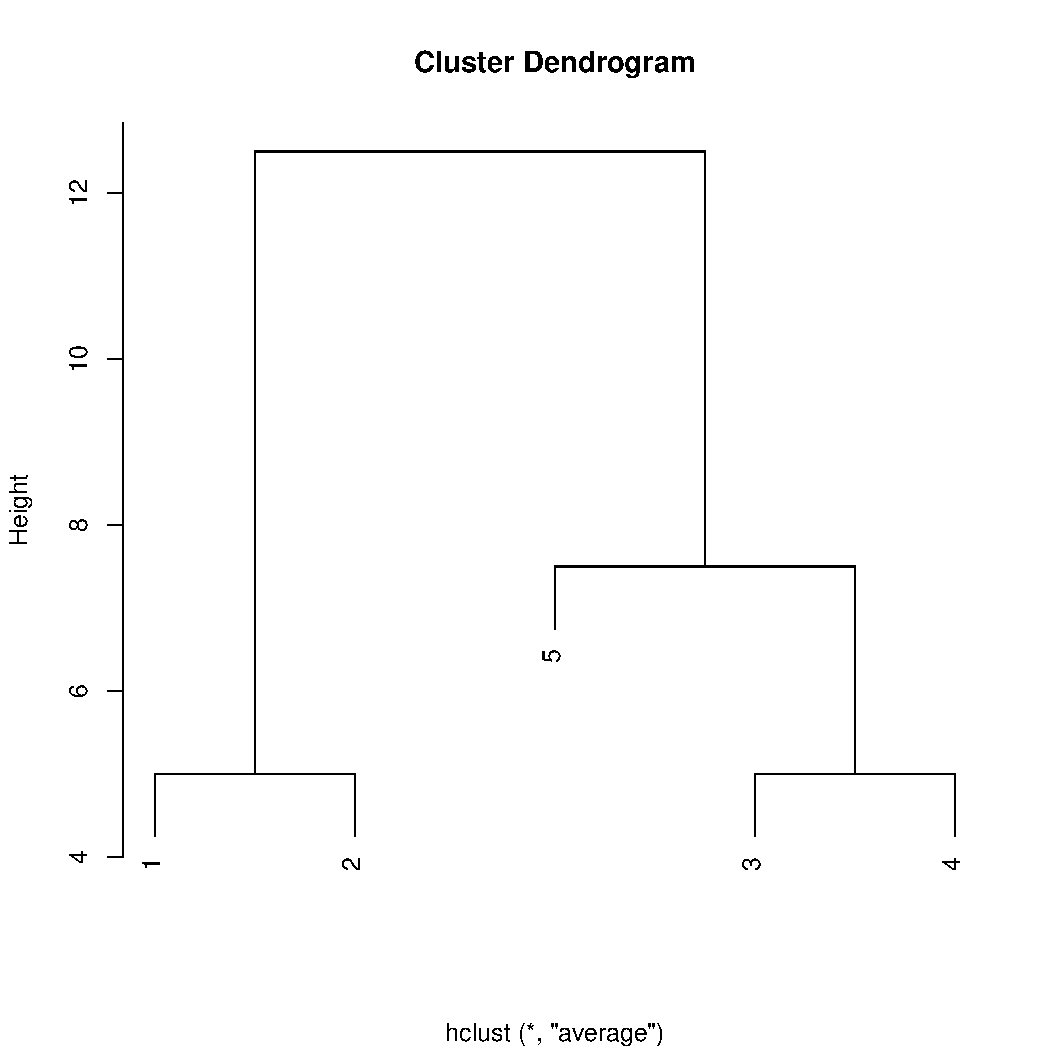
\includegraphics[width=\maxwidth]{figure/unnamed-chunk-3-1} 
\end{knitrout}

\end{document}
